\chapter{Test\index{Test}}
\label{chp:test}
\vspace*{-0.5em}
In this chapter, we conduct some tests in order to assess if using our process calculus for program parallelisation can help to yield a speedup. Furthermore, we are interested in whether there is a difference between the two implementations based on \textsf{Concurrent Haskell} and \textsf{Cloud Haskell}.

\section{Setup}
\vspace*{-0.5em}
For the tests, we use three variants of an artificial ant system that differ in their way of parallelisation but implement the same algorithm otherwise. One of the variants is the distributed ant system developed in \chpref{chp:ant_system_implementation}, we call it $A_{dis}$. $A_{con}$ is a slightly modified variant of $A_{dis}$ and uses the implementation of the developed process calculus that is based on \textsf{Concurrent Haskell} instead of \textsf{Cloud Haskell}. The third variant, $A_{seq}$, performs all computations sequentially and does not involve any parallelisation. The source code of all three variants can be found in \appref{app:dvd}.

As input for the ant systems, we use a set of 10 instances from the TSPLIB\footnote{The TSPLIB is a collection of instances of the \textsc{TSP} that have been solved to optimality and can be found at \url{http://www.iwr.uni-heidelberg.de/groups/comopt/software/TSPLIB95/tsp/}.}: \texttt{bays29}, \texttt{berlin52}, \texttt{st70}, \texttt{pr76}, \texttt{gr96}, \texttt{eil101}, \texttt{pr107}, \texttt{pr124}, \texttt{bier127} and \texttt{ch130}. The number included in the instance names give information about their size, i.e. the number of nodes in the graph described by the instance.

We configure the ant systems using parameters based on suggestions given in \cite{Dorigo:2004:ACO:975277}: $n$ ants for a graph of size $n$, $100$ iterations, initial pheromone concentration $\tau_0 = 2$, evaporation factor $\rho = 0.1$ and $\alpha = 2, \beta = 5$.

Since $A_{seq}$, $A_{con}$ and $A_{dis}$ are implementation of the same meta-heuristic and only differ in their parallelisation, we expect them to produce similar solutions in all cases. However, we're not interested in the proposed solutions but rather in the necessary time to obtain them. We use the runtime of $A_{seq}$ as a reference and compare the runtimes of $A_{con}$ and $A_{dis}$ against that.

The tests for comparing $A_{con}$ to $A_{seq}$ are carried out on an $\text{Intel}^{\textregistered}$ $\text{Core}^{\texttrademark}$ i7-3770 CPU @ 3.4GHz with 16GB RAM. We use \textsf{ghc} to compile the programs and the compiler flags \texttt{-O2} for $A_{seq}$ and \texttt{-threaded -O2} for $A_{con}$. We run $A_{con}$ with 1, 2, 3 and 4 cores active, using the \texttt{+RTS -N} option.

The tests for comparing $A_{dis}$ and $A_{seq}$ are carried out using a network of computers with $\text{Intel}^{\textregistered}$ $\text{Core}^{\texttrademark}$ i5-2400 CPUs @ 3.1GHz and 4GM RAM. We use \textsf{ghc} to compile the programs and the compiler flags \texttt{-O2} for $A_{seq}$ and \texttt{-threaded -O2} for $A_{dis}$. We run $A_{dis}$ with the dedicated master node on one computer and with 4, 8, 16 and 32 worker nodes connected. Note that, as the used CPUs have 4 physical cores, each of them can be used to run 4 worker nodes.

\vspace*{-1em}
\section{Results}
The results of the test runs for the comparison of $A_{seq}$ and $A_{con}$ are shown in table \ref{tbl:test1} and visualised in \figref{fig:test1}. Analogously, the results for the comparison of $A_{seq}$ and $A_{dis}$ are shown in table \ref{tbl:test2} and visualised in \figref{fig:test2}. Unreasonably high values are not shown in the plot.

\vspace*{-1em}

\begin{table}[h!]
  \centering
  \begin{tabular}{r|c||c|c|c|c|}
    \cline{2-6}
    & \multicolumn{1}{c||}{$A_{seq}$} & \multicolumn{4}{c|}{$A_{con}$} \\
    \hline
    \multicolumn{1}{|r||}{scenario} & & 1 core & 2 cores & 3 cores & 4 cores \\
    \hline
    \hline
    \multicolumn{1}{|r||}{\texttt{bays29}} & 0.45s & 0.511s & 0.424s & 0.379s & 0.375s \\
    \hline
    \multicolumn{1}{|r||}{\texttt{berlin52}} & 2.253s & 2.561s & 2.016s & 1.657s & 1.521s \\
    \hline
    \multicolumn{1}{|r||}{\texttt{st70}} & 5.292s & 6.484s & 4.911s & 3.894s & 3.416s \\
    \hline
    \multicolumn{1}{|r||}{\texttt{pr76}} & 6.4s & 8.546s & 6.142s & 4.867s & 4.236s \\
    \hline
    \multicolumn{1}{|r||}{\texttt{gr96}} & 12.855s & 20.767s & 13.703s & 9.881s & 8.209s \\
    \hline
    \multicolumn{1}{|r||}{\texttt{eil101}} & 15.126s & 25.893s & 16.682s & 11.949s & 9.773s \\
    \hline
    \multicolumn{1}{|r||}{\texttt{pr107}} & 16.244s & 26.738s & 16.482s & 11.817s & 10.521s \\
    \hline
    \multicolumn{1}{|r||}{\texttt{pr124}} & 26.277s & 50.024s & 30.203s & 22.587s & 18.33s \\
    \hline
    \multicolumn{1}{|r||}{\texttt{bier127}} & 28.468s & 54.311s & 33.37s & 24.948s & 20.225s \\
    \hline
    \multicolumn{1}{|r||}{\texttt{ch130}} & 32.039s & 61.328s & 37.042s & 27.866s & 22.909s \\
    \hline
  \end{tabular}
  \caption{Runtimes of $A_{seq}$ and $A_{con}$ on an $\text{Intel}^{\textregistered}$ $\text{Core}^{\texttrademark}$ i7-3770 CPU @ 3.4GHz with 16GB RAM.}
  \vspace*{-0.75em}
  \label{tbl:test1}
\end{table}

\begin{figure}[h!]
  \centering
  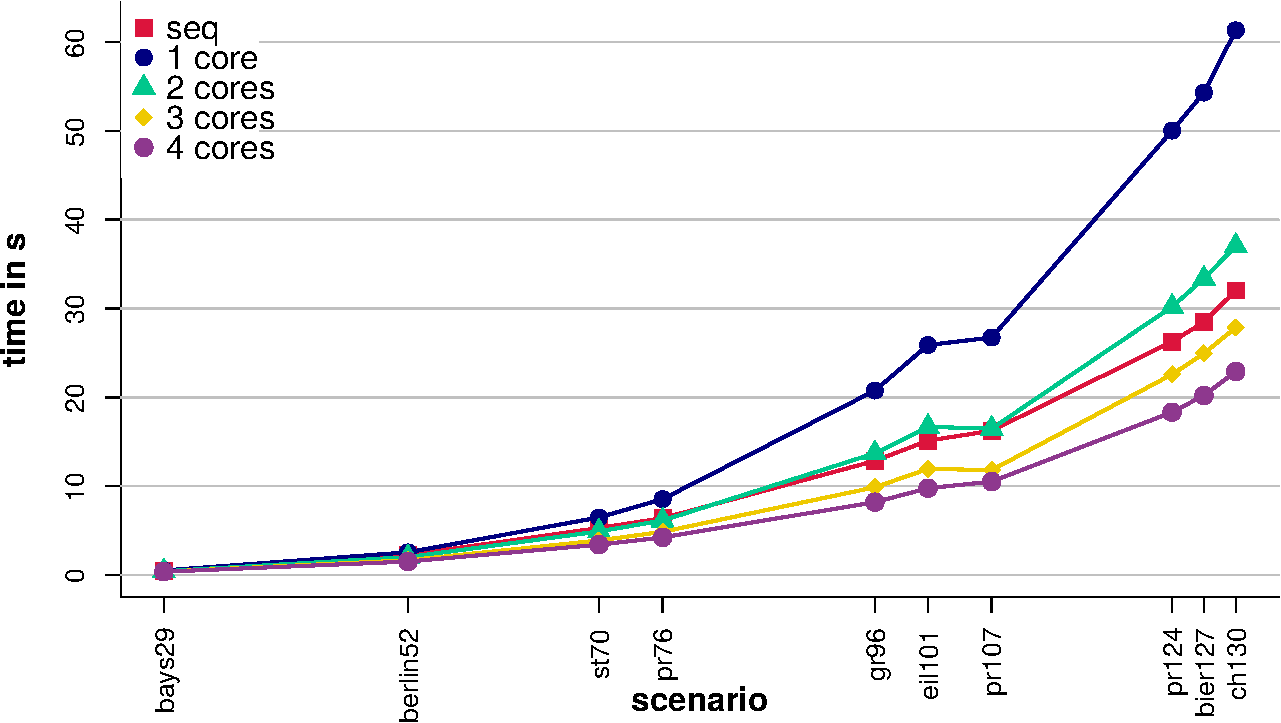
\includegraphics[width=\textwidth]{img/test_local.pdf}
  \caption{The runtimes of $A_{seq}$ and $A_{con}$ based on the data from table \ref{tbl:test1}.}
  \label{fig:test1}
\end{figure}

\begin{table}[h!]
  \centering
  \begin{tabular}{r|c||c|c|c|c|c|}
    \cline{2-7}
    & \multicolumn{1}{c||}{$A_{seq}$} & \multicolumn{5}{c|}{$A_{dis}$} \\
    \hline
    \multicolumn{1}{|r||}{scenario} & & 4 worker & 8 worker & 16 worker & 32 worker & 64 worker \\
    \hline
    \hline
    \multicolumn{1}{|r||}{\texttt{bays29}} & 0.558s & 57s & 39s & 28s & 30s & 29s \\
    \hline
    \multicolumn{1}{|r||}{\texttt{berlin52}} & 2.939s & 146s & 97s & 72s & 63s & 61s \\
    \hline
    \multicolumn{1}{|r||}{\texttt{st70}} & 6.844s & 282s & 189s & 137s & 119s & 108s \\
    \hline
    \multicolumn{1}{|r||}{\texttt{pr76}} & 10.751s & 355s & 233s & 162s & 138s & 128s \\
    \hline
    \multicolumn{1}{|r||}{\texttt{gr96}} & 16.692s & 629s & 448s & 306s & 247s & 223s \\
    \hline
    \multicolumn{1}{|r||}{\texttt{eil101}} & 19.515s & 771s & 515s & 353s & 281s & 252s \\
    \hline
    \multicolumn{1}{|r||}{\texttt{pr107}} & 21.474s & 866s & 586s & 407s & 325s & 295s \\
    \hline
    \multicolumn{1}{|r||}{\texttt{pr124}} & 34.469s & 1,342s & 864s & 603s & 480s & 427s \\
    \hline
    \multicolumn{1}{|r||}{\texttt{bier127}} & 39.341s & 1,364s & 937s & 647s & 515s & 460s \\
    \hline
    \multicolumn{1}{|r||}{\texttt{ch130}} & 41.225s & 1,472s & 1,002s & 699s & 547s & 495s \\
    \hline
  \end{tabular}
  \caption{Runtimes of $A_{seq}$ and $A_{dis}$ in a network of computers with $\text{Intel}^{\textregistered}$ $\text{Core}^{\texttrademark}$ i5-2400 CPUs @ 3.1GHz and 4GM RAM.}
  \vspace*{-0.75em}
  \label{tbl:test2}
\end{table}

\begin{figure}[h!]
  \centering
  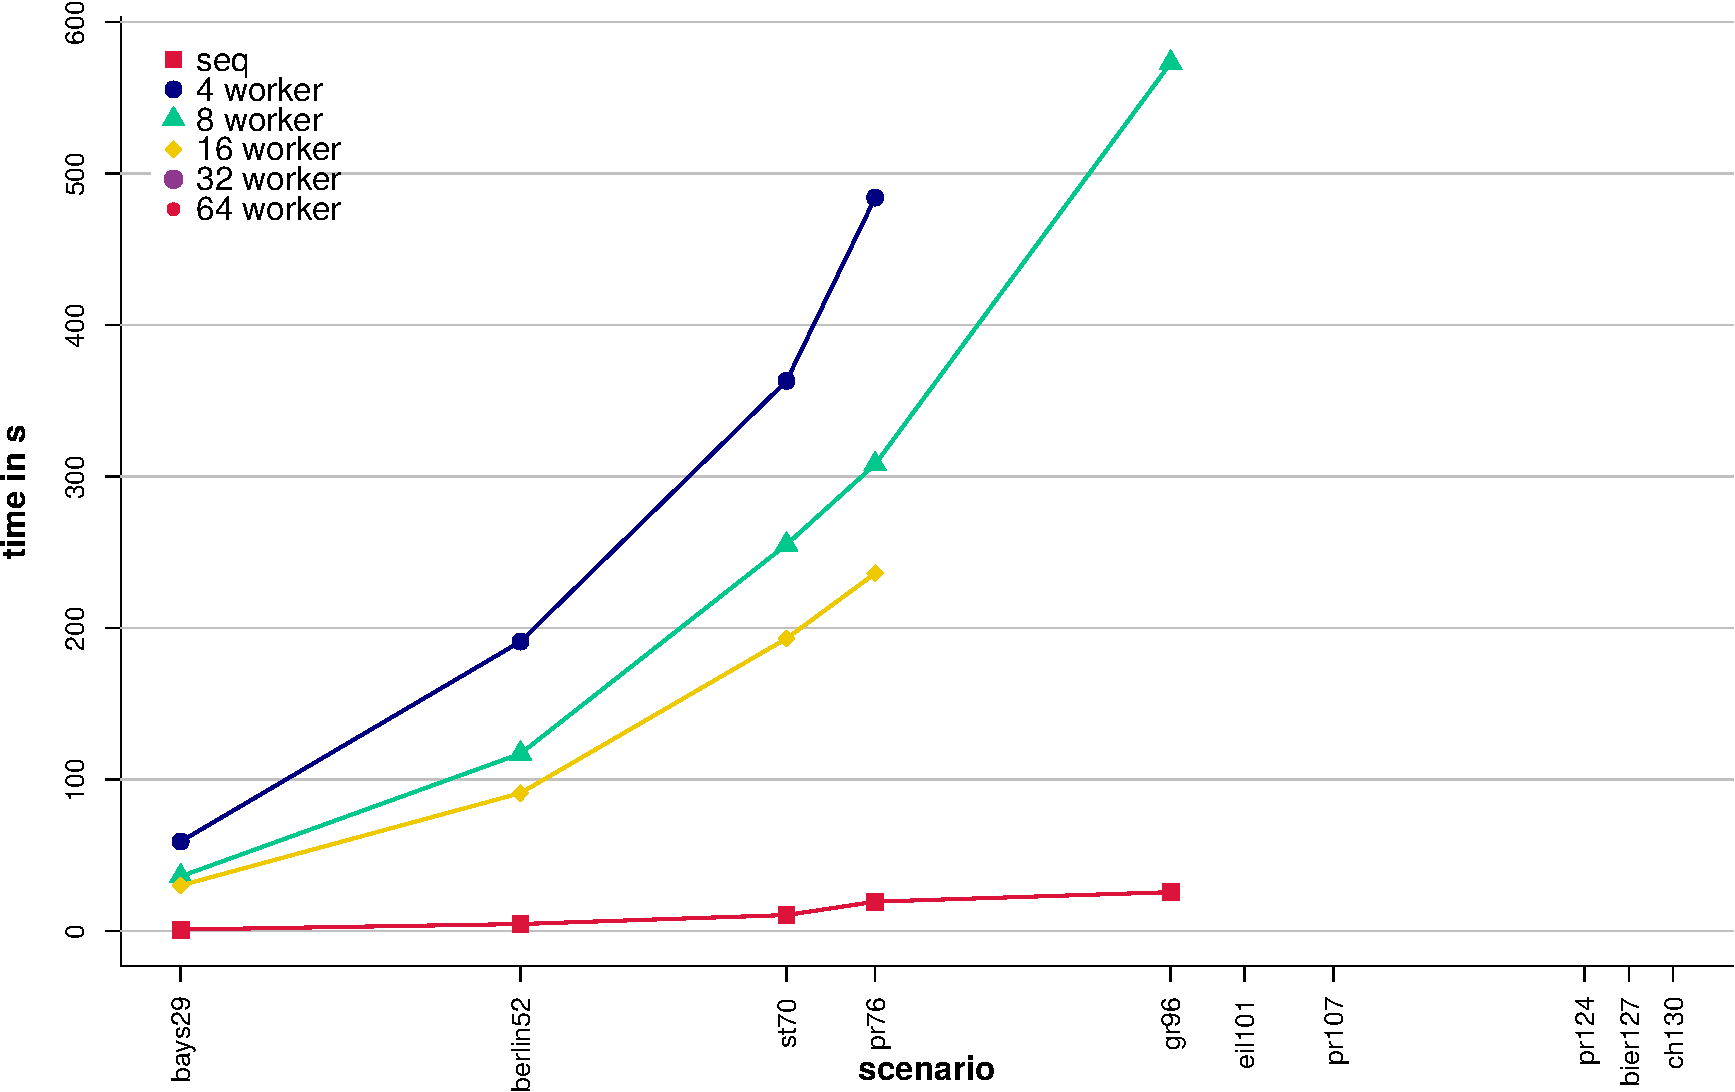
\includegraphics[width=\textwidth]{img/test_distributed.pdf}
  \caption{The runtimes of $A_{seq}$ and $A_{dis}$ based on the data from table \ref{tbl:test2}.}
  \label{fig:test2}
\end{figure}

\clearpage
\section{Interpretation}
The test results show that in general, a speedup can be achieved when using the developed process calculus for program parallelisation. The runtime of $A_{con}$ decreases as there are more physical cores made available to carry out the computations. A similar behaviour can be observed for $A_{dis}$: the more worker nodes are connected, the faster a solution can be computed, the system scales.

However, when put into relation to the runtime of $A_{seq}$ on the respective hardware, $A_{con}$ and $A_{dis}$ show different properties. Depending on the scenario, $A_{con}$ achieves a speedup between $1.2$ and $1.57$ compared to $A_{seq}$ when 4 cores are used. Contrary to the expectation, $A_{dis}$ is not able to achieve a speedup compared to $A_{seq}$, but takes between $11.69$ and $51.97$ times as long as $A_{seq}$, even with 64 worker nodes connected, depending on the scenario.

The data shows that $A_{con}$ takes between $1.14$ and $1.91$ times as long as $A_{seq}$ to find solutions when only using one core. This may be explained with the introduced overhead for expressing parallelism using our process calculus and interpreting the process structures. Depending on the scenario, $A_{con}$ needs 2 or 3 cores to be able to outperform $A_{seq}$. We expect that $A_{con}$ could perform even faster with more than 4 cores, however one should not forget that the sequential part of the program gives an upper bound for the maximum achievable speedup as stated by \textsc{Amdahl}'s law.

In our tests, $A_{dis}$ was not able to outperform $A_{seq}$, no matter how many workers are connected. In order to explain this, different things may have to be taken into account. On the one hand, the process interpreter has to request a worker node for every process from the master node and wait for the reply. Since network communication takes remarkably longer than forking a local thread, a much higher overhead is introduced in $A_{dis}$ than in $A_{con}$. On the other hand, for every process that is spawned remotely, a function closure has to be serialised, sent to a remote node and deserialised there. Before termination, the remote process has to serialise its result and send it back to the caller. This way of making data available to the processes takes remarkably longer than shared access to the memory as is the case in $A_{con}$. It is left open for future work to investigate in the reasons for this.